\documentclass[12pt,UTF8]{ctexart}
\usepackage{ctex,amsmath,amssymb,geometry,fancyhdr,bm,amsfonts
,mathtools,extarrows,graphicx,url,enumerate,color,float,multicol,rotating,subfig} 
\allowdisplaybreaks[4]
% 加入中文支持
\newcommand\Set[2]{\{#1\ \vert\ #2 \}}
\newcommand\Lim[0]{\lim\limits_{n\rightarrow\infty}}
\newcommand\LIM[2]{\lim\limits_{#1\rightarrow#2}}
\newcommand\Ser[1]{\sum_{n=#1}^\infty}
\newcommand{\SER}[2]{\sum_{#1=#2}^\infty}
\newcommand{\Int}[4]{\int_{#1}^{#2}#3\mathrm d#4}
\newcommand{\md}[0]{\mathrm d}
\geometry{a4paper,scale=0.80}
\pagestyle{fancy}
\rhead{多元函数微分学的应用(1)}
\lhead{基础习题课期末复习}
\chead{微积分B(2)}
\begin{document}
\setcounter{section}{3}
\section{几何应用}
\noindent
\subsection{复习计划}
\begin{figure}[H]
\begin{center}
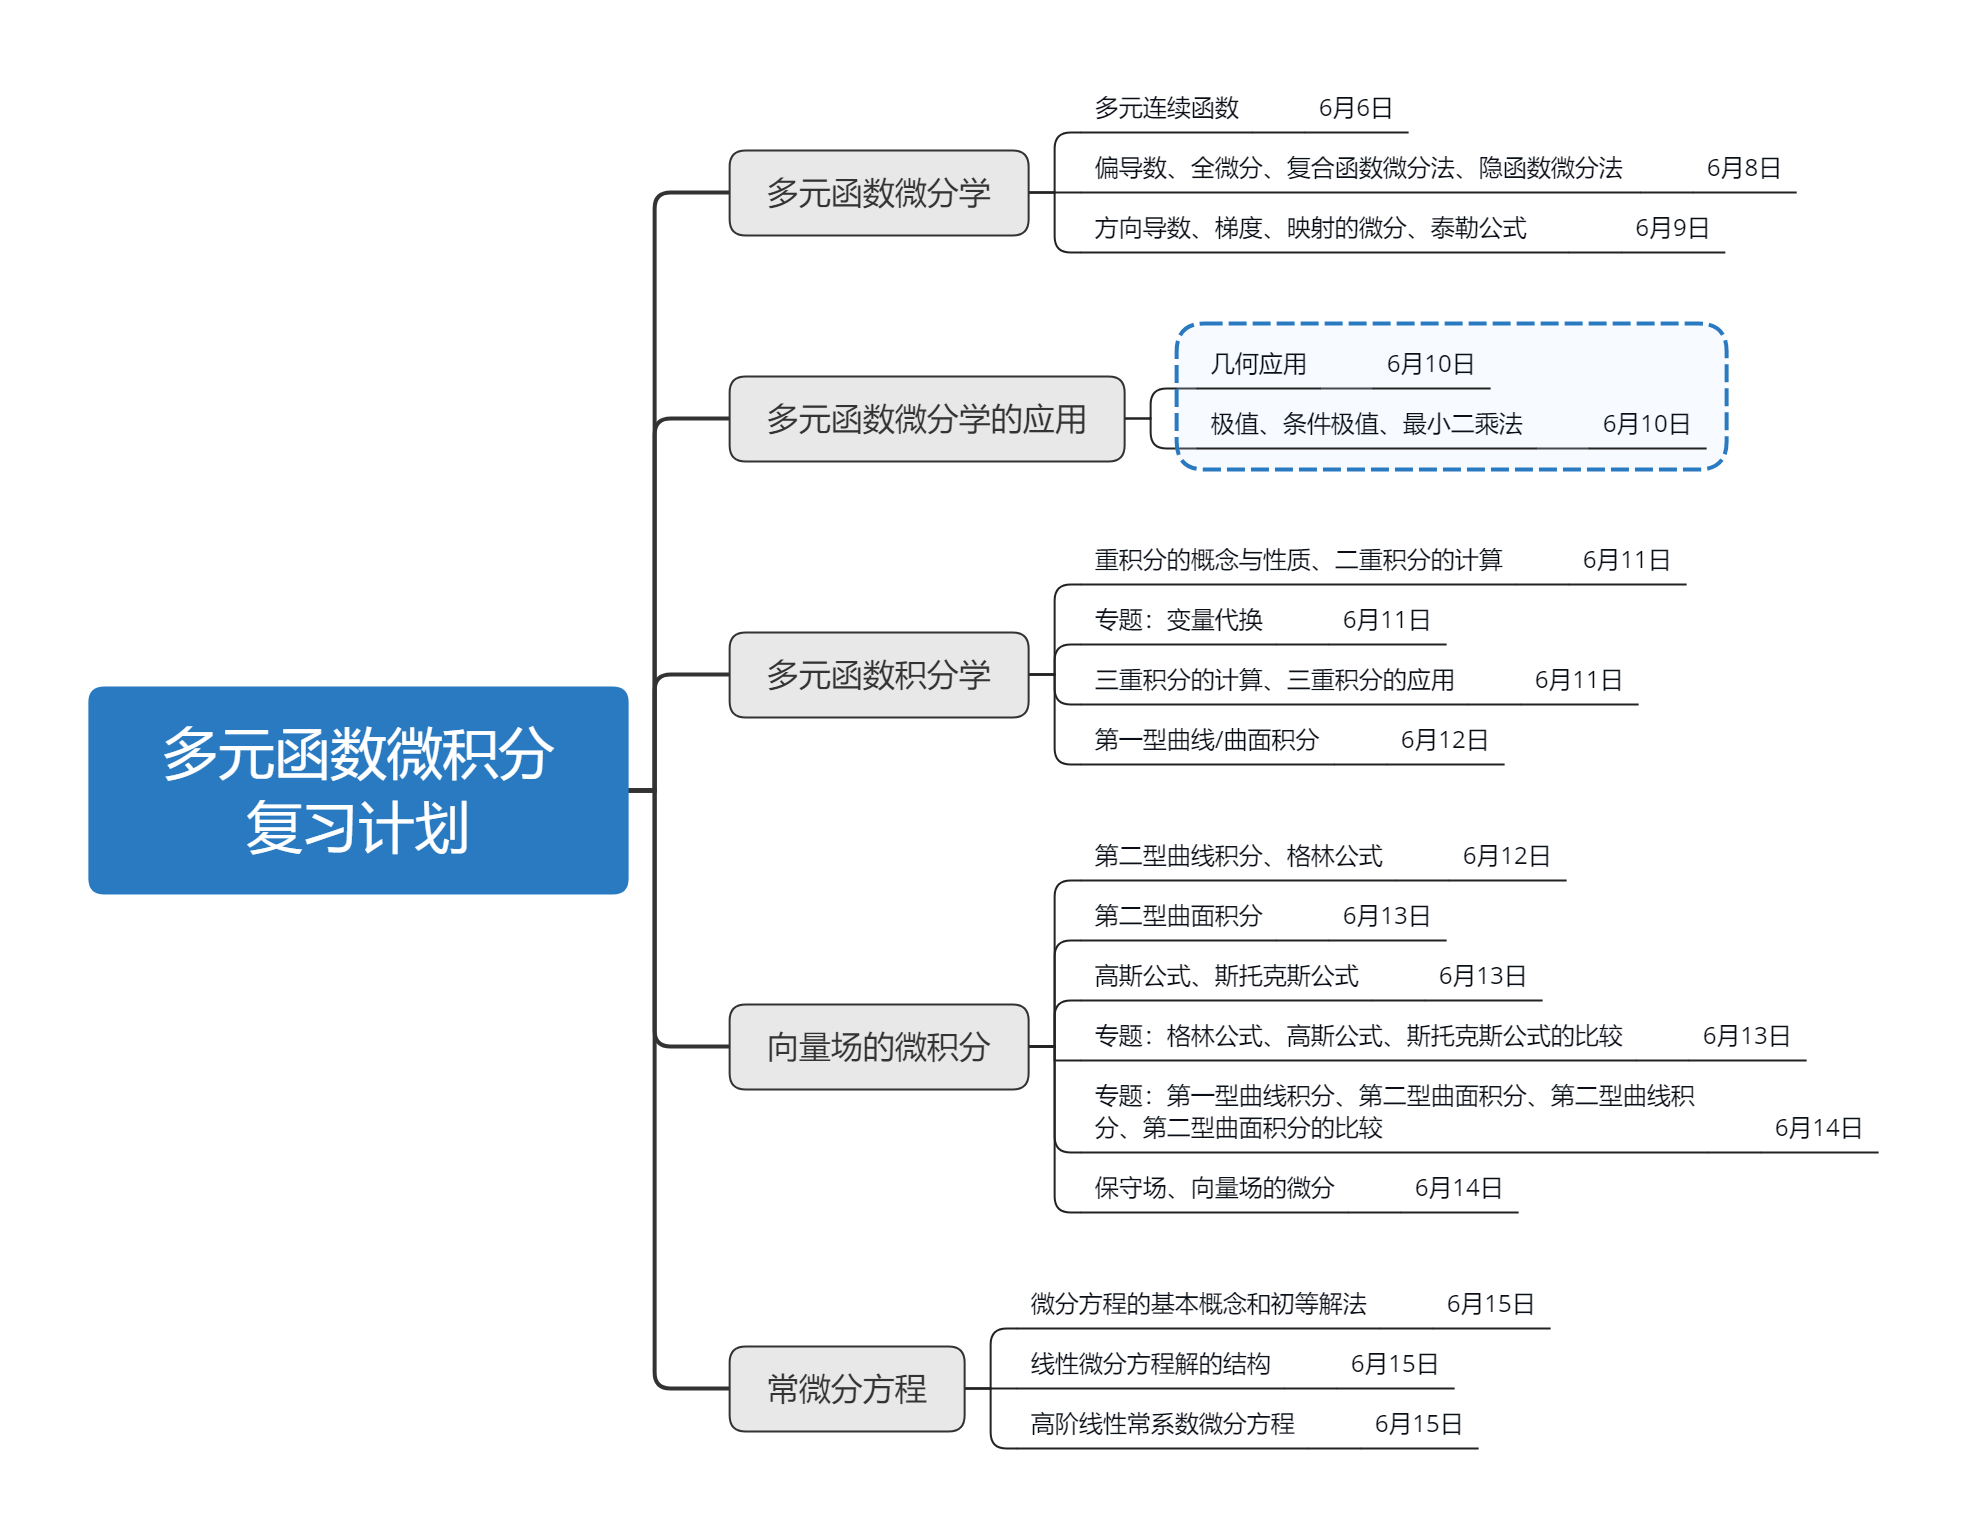
\includegraphics[height=0.5\textheight]{Figures20190610/plan.png}
\end{center}
\end{figure}
\subsection{知识结构}
\begin{figure}[H]
\begin{center}
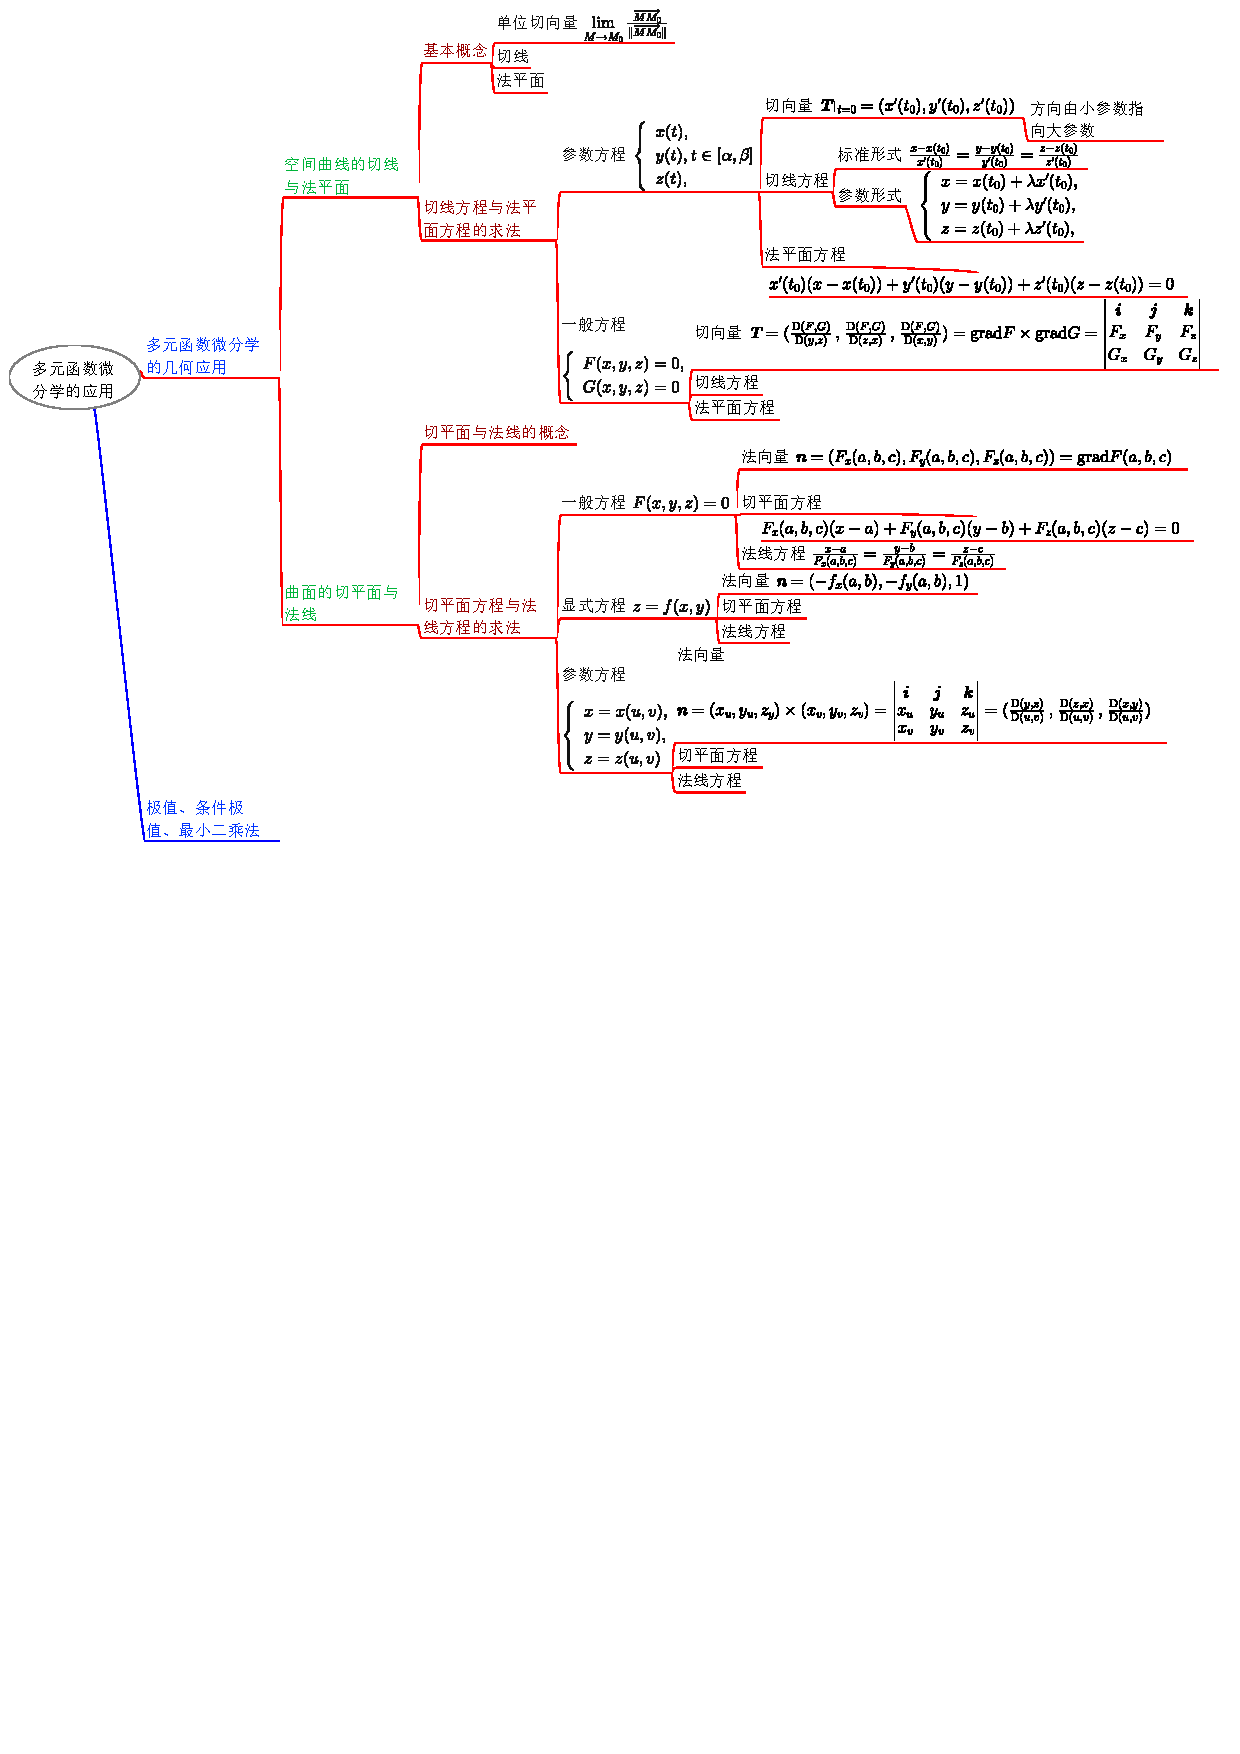
\includegraphics[height=0.9\textheight,angle=0]{20190610.pdf}
\end{center}
\end{figure}
\subsection{重要知识}
\begin{enumerate}
\item切平面的图示.
\begin{figure}[H]
\begin{center}
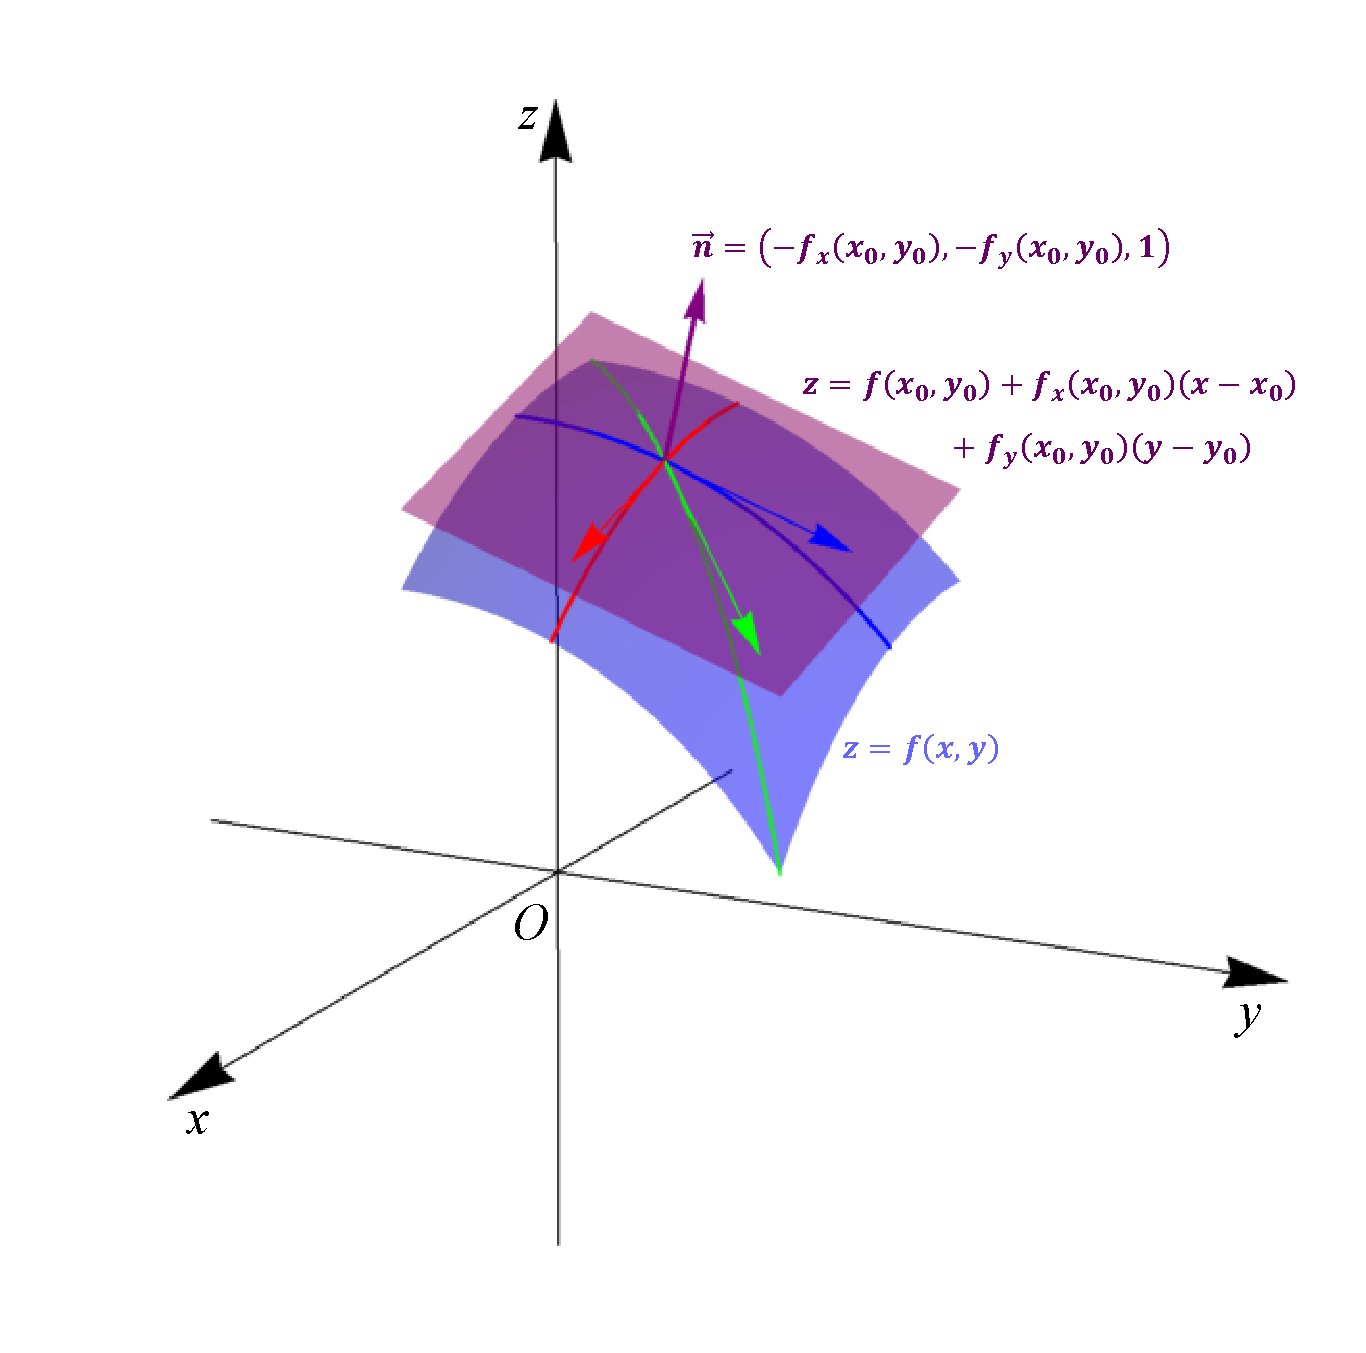
\includegraphics[height=0.7\textheight]{Figures20190610/tangentsurface.pdf}
\end{center}
\caption{切平面的图示}
\end{figure}
\end{enumerate}
\subsection{习题分类与解题思路}
\begin{enumerate}
\item已知曲线的参数方程,求切向量或切线方程. 可直接代入公式计算.

【如习题11.1中的2., 3., 7., 8.】
\item求曲面的切平面和法线方程,可分成以下情况,代入公式求解.
\begin{enumerate}
\item已知一般(隐式)方程或显式方程.

【如习题11.2中的1.(1)/(2)/(3)/(4), 4.】
\item已知参数方程.

【如习题11.2中的1.(5), 2.(3).】
\end{enumerate}
\item求曲面的满足一定要求的切平面方程.
\begin{enumerate}
\item求曲面上与已知平面平行的切平面. 法向量已知,关键是求切点. 注意椭球面有两个切点.

【如习题11.2中的2.(1).】
\item求曲面上与已知直线垂直的切平面. 需求出直线的方向向量,等于切平面的法向量,进一步可求切点. 

【如习题11.2中的2.(2).】
\end{enumerate}
\item证明曲面的全体切平面满足特殊关系. 可先利用公式求出曲面的全体切平面方程,结合要证明的结论对方程进行化简.

【如习题11.2中的3., 5., 6.】
\item其他类型的题目. 大家可以做一下积累.

【习题11.2中的7., 8.】
\end{enumerate}
\subsection{习题11.1解答}
\begin{enumerate}
\item[2.]求下列曲线在指定点的单位切向量:\\
(1)$\bm r(t)=(\mathrm e^{2t},\mathrm e^{-2t},t\mathrm e^{2t}),t=0$;\\
(2)$\bm r(t)=t\bm i+2\sin t\bm j+3\cos t\bm k,t=\frac\pi6$.

解:(1)单位切向量$\bm t=\frac{\bm r'(t)}{|\bm r'(t)|}=\frac{(2\mathrm e^{2t},-2\mathrm e^{-2t},(1+2t)\mathrm e^{2t})}{\|(2\mathrm e^{2t},-2\mathrm e^{-2t},(1+2t)\mathrm e^{2t})\|}\Big|_{t=0}=\frac{(2,-2,1)}{\sqrt{4+4+1}}=(\frac23,-\frac23,\frac13)$.

(2)单位切向量$\bm t=\frac{\bm r'(t)}{|\bm r'(t)|}=\frac{\bm i+2\cos t\bm j-3\sin t\bm k}{\|\bm i+2\cos t\bm j-3\sin t\bm k\|}\Big|_{t=\frac\pi6}=\frac{\bm i+\sqrt3\bm j-\frac32\bm k}{\sqrt{1+3+\frac94}}=\frac25\bm i+\frac{2\sqrt3}5\bm j-\frac35\bm k$.

\item[3.]求下列曲线在指定点的切线方程:\\
(1)$\bm r(t)=(1+2t,1+t-t^2,1-t+t^2-t^3),M(1,1,1)$;\\
(2)$\bm r(t)=\sin(\pi t)\bm i+\sqrt t\bm j+\cos(\pi t)\bm k,M(0,1,-1)$.

解:(1)在$M(1,1,1)$点处$t=0$,切向量$\bm t=\bm r'(0)=(2,1-2t,-1+2t-3t^2)_{t=0}=(2,1,-1)$,则切线方程为
\[\frac{x-1}2=y-1=-(z-1).\]
(2)在$M(0,1,-1)$点处$t=1$,切向量$\bm t=\bm r'(1)=\pi\cos(\pi t)\bm i+\frac1{2\sqrt t}\bm j-\pi\sin(\pi t)\bm k\big|_{t=1}=-\pi\bm i+\frac12\bm j$,则切线方程为$\begin{cases}
\frac x{-\pi}=2(y-1),\\
z=-1,
\end{cases}$即$\begin{cases}
x+2\pi y=2\pi,\\
z=-1.
\end{cases}$

\item[7.]求等速圆周运动$\bm r=R\cos(\omega t)\bm i+R\sin(\omega t)\bm j$在$t$时刻的速度与加速度.

解:$t$时刻的速度$\bm v(t)=\bm r'(t)=-R\omega\sin(\omega t)\bm i+R\omega\cos(\omega t)\bm j$,

$t$时刻的加速度$\bm a(t)=\bm v'(t)=-R\omega^2\cos(\omega t)\bm i-R\omega^2\sin(\omega t)\bm j$.

\item[8.]已知螺旋线的向量方程为$\bm r=a\cos\theta\bm i+a\sin\theta\bm j+b\theta\bm k(a>0,b>0)$,求在$\theta_0$处的切线方程.

解:在$\theta_0$处的切向量$\bm r'(\theta_0)=-a\sin\theta_0\bm i+a\cos\theta_0\bm j+b\bm k$,切线方程
\[\frac{x-a\cos\theta_0}{-a\sin\theta_0}=\frac{y-a\sin\theta_0}{a\cos\theta_0}=\frac{z-b\theta_0}b.\]
\end{enumerate}
\subsection{习题11.2解答}
\begin{enumerate}
\item求下列曲面在指定点的法线方程与切平面的方程:\\
(1)$x^2+y^2+z^2=14$,在点$(1,2,3)$;\\
(2)$z=\frac12x^2-y^2$,在点$(2,-1,1)$;\\
(3)$(2a^2-z^2)x^2-a^2y^2=0$,在点$(a,a,a)$;\\
(4)$\frac{x^2}{a^2}+\frac{y^2}{b^2}+\frac{z^2}{c^2}=1$,在点$(\frac a{\sqrt3},\frac b{\sqrt3},\frac c{\sqrt3})$;\\
(5)$\begin{cases}
x=u\cos v,\\
y=u\sin v,\\
z=av,
\end{cases}$在$(u,v)=(u_0,v_0)$处.

解:(1)法向量$\bm n=(2x,2y,2z)\big|_{(1,2,3)}=2(1,2,3)$,

法线方程$x-1=\frac{y-2}2=\frac{z-3}3$,

切平面方程$(x-1)+2(y-2)+3(z-3)=0$,即$x+2y+3z=14$.

(2)法向量$\bm n=(x,-2y,-1)\big|_{(2,-1,1)}=(2,2,-1)$,

法线方程$\frac{x-2}2=\frac{y+1}2=-(z-1)$,

切平面方程$2(x-2)+2(y+1)-(z-1)=0$,即$2x+2y-z=1$.

(3)法向量$\bm n=(2(2a^2-z^2)x,-2a^2y,-2x^2z)\big|_{(a,a,a)}=2a^3(1,-1,-1)$,

法线方程$x-a=-(y-a)=-(z-a)$,

切平面方程$(x-a)-(y-a)-(z-a)=0$,即$x-y-z=-a$.

(4)法向量$\bm n=(\frac{2x}{a^2},\frac{2y}{b^2},\frac{2z}{c^2})\big|_{(\frac a{\sqrt3},\frac b{\sqrt3},\frac c{\sqrt3})}=\frac2{\sqrt3}(\frac1a,\frac1b,\frac1c)$,

法线方程$a(x-\frac a{\sqrt3})=b(y-\frac b{\sqrt3})=c(z-\frac c{\sqrt3})$,

切平面方程$\frac1a(x-\frac a{\sqrt3})+\frac1b(y-\frac b{\sqrt3})+\frac1c(z-\frac c{\sqrt3})=0$,即$\frac xa+\frac yb+\frac zc=\sqrt3$.

(5)法向量$\bm n=(\cos v,\sin v,0)\times(-u\sin v,u\cos v,a)\big|_{(u_0,v_0)}=\begin{vmatrix}
\bm i&\bm j&\bm k\\
\cos v_0&\sin v_0&0\\
-u_0\sin v_0&u_0\cos v_0&a
\end{vmatrix}\\
=(\begin{vmatrix}
\sin v_0&0\\
u_0\cos v_0&a
\end{vmatrix},\begin{vmatrix}
0&a\\
a&u_0\cos v_0
\end{vmatrix},\begin{vmatrix}
\cos v_0&\sin v_0\\
-u_0\sin v_0&u_0\cos v_0
\end{vmatrix})=(a\sin v_0,-a\cos v_0,u_0)$,

法线方程$\frac{x-u_0\cos v_0}{a\sin v_0}=\frac{y-u_0\sin v_0}{-a\cos v_0}=\frac{z-av_0}{u_0}$,

切平面方程$a\sin v_0(x-u_0\cos v_0)-a\cos v_0(y-u_0\sin v_0)+u_0(z-av_0)=0$,\\
即$ax\sin v_0-ay\cos v_0+zu_0=au_0v_0$.

\item按要求求下列曲面的切平面方程:\\
(1)曲面$x^2+2y^2+3z^2=21$的与平面$x+4y+6z=0$平行的切平面;\\
(2)曲面$z=x^2+y^2$的与直线$\begin{cases}
x+2z=1,\\
y+2z=2
\end{cases}$垂直的切平面;\\
(3)双曲抛物面$\bm r=(u+v,u-v,uv)$在$u=1,v=-1$处的切平面.

解:(1)曲面的法向量$\bm n=(2x,4y,6z)$,平面的法向量$\bm n_1=(1,4,6)$,\\则由$\begin{cases}(2x,4y,6z)=a(1,4,6),\\
x^2+2y^2+3z^2=21
\end{cases}$得曲面上与该平面相切的切平面的切点为$\pm(1,2,2)$,

切平面方程$x-1+4(y-2)+6(z-2)=0$或$x+1+4(y+2)+6(z+2)=0$,即$x+4y+6z=\pm21$.

(2)直线的切向量$\bm t=(1,0,2)\times(0,1,2)=\begin{vmatrix}
\bm i&\bm j&\bm k\\
1&0&2\\
0&1&2\\
\end{vmatrix}=(\begin{vmatrix}
0&2\\
1&2
\end{vmatrix},\begin{vmatrix}
2&1\\
2&0
\end{vmatrix},\begin{vmatrix}
1&0\\
0&1
\end{vmatrix})=(-2,-2,1)$,曲面的法向量$\bm n=(2x,2y,-1)$,曲面上与直线垂直的切平面的法向量$\bm n_0=a\bm t$,\\
由$\begin{cases}
(2x,2y,-1)=a(-2,-2,1),\\
z=x^2+y^2
\end{cases}$可得切点为$(1,1,2)$,

切平面方程$-2(x-1)-2(y-1)+z-2=0$,即$2x+2y-z=2$.

(3)法向量$\bm n=(1,1,v)\times(1,-1,u)\big|_{(1,-1)}=\begin{vmatrix}
\bm i&\bm j&\bm k\\
1&1&-1\\
1&-1&1
\end{vmatrix}=(\begin{vmatrix}
1&-1\\
-1&1
\end{vmatrix},\begin{vmatrix}
-1&1\\
1&1
\end{vmatrix},\begin{vmatrix}
1&1\\
1&-1
\end{vmatrix})\\
=(0,-2,-2)$,切点为$(0,2,-1)$,

切平面的方程$-2(y-2)-2(z+1)=0$,即$y+z=1$.

\item求证:曲面$\sqrt x+\sqrt y+\sqrt z=\sqrt a,a>0$在任意点处的切平面在各坐标轴上的截距之和为$a$.

证明:曲面在任意点$(x_0,y_0,z_0)$处的法向量$\bm n=\frac12(\frac1{\sqrt{x_0}},\frac1{\sqrt{y_0}},\frac1{\sqrt{z_0}})$,\\
切平面方程$\frac1{\sqrt{x_0}}(x-x_0)+\frac1{\sqrt{y_0}}(y-y_0)+\frac1{\sqrt{z_0}}(z-z_0)=0$,即$\frac x{ax_0}+\frac y{ay_0}+\frac z{az_0}=1$,

切平面在$x,y,z$轴上的截距之和
\[\begin{split}
\sqrt{ax_0}+\sqrt{ay_0}+\sqrt{az_0}=\sqrt a(\sqrt{x_0}+\sqrt{y_0}+\sqrt{z_0})=a.
\end{split}\]

\item证明二次曲面$ax^2+by^2+cz^2=1$在点$M_0(x_0,y_0,z_0)$处的切平面方程为
\[
ax_0x+by_0y+cz_0z=1.
\]
证明:曲面在点$M_0(x_0,y_0,z_0)$处的法向量$\bm n=2(ax_0,by_0,cz_0)$,

切平面方程
\[\begin{split}
&ax_0(x-x_0)+by_0(y-y_0)+cz_0(z-z_0)\\
=&ax_0x-ax_0^2+by_0y-by_0^2+cz_0z-cz_0^2\\
=&ax_0x-by_0y-cz_0z-1=0,
\end{split}\]
即\[
ax_0x+by_0y+cz_0z=1.
\]

\item设函数$f$可微,试证曲面$z=yf(\frac xy)$的所有切平面相交于一个公共点.

证明:曲面在点$(x_0,y_0,z_0)$处的法向量$\bm n=(yf'(\frac xy)\frac1y,f(\frac xy)+yf'(\frac xy)(-\frac x{y^2}),-1)\big|_{(x_0,y_0,z_0)}\\
=(f'(\frac{x_0}{y_0}),f(\frac{x_0}{y_0})-\frac{x_0}{y_0}f'(\frac{x_0}{y_0}),-1)$,

切平面的方程
\[\begin{split}
&f'(\frac{x_0}{y_0})(x-x_0)+[f(\frac{x_0}{y_0})-\frac{x_0}{y_0}f'(\frac{x_0}{y_0})](y-y_0)-(z-z_0)\\
=&f'(\frac{x_0}{y_0})x+[f(\frac{x_0}{y_0})-\frac{x_0}{y_0}f'(\frac{x_0}{y_0})]y-z-x_0f'(\frac{x_0}{y_0})-y_0f(\frac{x_0}{y_0})+x_0f'(\frac{x_0}{y_0})+z_0\\
=&f'(\frac{x_0}{y_0})x+[f(\frac{x_0}{y_0})-\frac{x_0}{y_0}f'(\frac{x_0}{y_0})]y-z\\
%=&f'(\frac{x_0}{y_0})(x-\frac{x_0}{y_0}y)+f(\frac{x_0}{y_0})y-z\\
%=&f'(\frac{x_0}{y_0})(x-\frac{x_0}{y_0}y)+\frac{z_0}{y_0}y-z\\
=&0,
\end{split}\]
$\because$无论切点$(x_0,y_0,z_0)$取在何处,点$(x,y,z)=(0,0,0)$始终满足以上方程,

$\therefore$曲面$z=yf(\frac xy)$的所有切平面相交于一个公共点$(0,0,0)$.

\item已知函数$f$可微,证明曲面$f(\frac{x-a}{z-c},\frac{y-b}{z-c})=0$上任意一点处的切平面通过一定点,并求出此点的位置.

证明:曲面上任一点$(x_0,y_0,z_0)$处的法向量
\[
\bm n=(\frac1{z_0-c}f'_1,\frac1{z_0-c}f'_2,-\frac{x_0-a}{(z_0-c)^2}f'_1-\frac{y_0-b}{(z_0-c)^2}f'_2),
\]
切平面方程
\[\begin{split}
&\frac{x-x_0}{z_0-c}f'_1+\frac{y-y_0}{z_0-c}f'_2+[-\frac{x_0-a}{(z_0-c)^2}f'_1-\frac{y_0-b}{(z_0-c)^2}f'_2](z-z_0)\\
=&[\frac{x-x_0}{z_0-c}-\frac{x_0-a}{(z_0-c)^2}(z-z_0)]f'_1+[\frac{y-y_0}{z_0-c}-\frac{y_0-b}{(z_0-c)^2}(z-z_0)]f'_2\\
=&0,
\end{split}\]
其中偏导数均在$(\frac{x_0-a}{z_0-c},\frac{y_0-b}{z_0-c})$处取值,

$\because$无论切点$(x_0,y_0,z_0)$取在何处,$(x,y,z)=(a,b,c)$始终满足以上方程,

$\therefore$曲面$f(\frac{x-a}{z-c},\frac{y-b}{z-c})=0$上任意一点处的切平面通过定点$(a,b,c)$.

\item设曲面$S_1$和$S_2$的方程分别为$F_1(x,y,z)=0,F_2(x,y,z)=0$,其中$F_1$和$F_2$是可微函数,试证$S_1$与$S_2$垂直的充分必要条件是对交线上的任意一点$(x,y,z)$,均有
\[
\frac{\partial F_1}{\partial x}\frac{\partial F_2}{\partial x}+\frac{\partial F_1}{\partial y}\frac{\partial F_2}{\partial y}+\frac{\partial F_1}{\partial z}\frac{\partial F_2}{\partial z}=0.
\]
证明:必要性:$\because S_1$与$S_2$垂直,

$\therefore$交线上的任意一点$(x,y,z)$处两曲面的法向量互相垂直,即
\[
(\frac{\partial F_1}{\partial x},\frac{\partial F_1}{\partial y},\frac{\partial F_1}{\partial z})\bm\cdot(\frac{\partial F_2}{\partial x},\frac{\partial F_2}{\partial y},\frac{\partial F_2}{\partial z})=\frac{\partial F_1}{\partial x}\frac{\partial F_2}{\partial x}+\frac{\partial F_1}{\partial y}\frac{\partial F_2}{\partial y}+\frac{\partial F_1}{\partial z}\frac{\partial F_2}{\partial z}=0;
\]
充分性:$\because$交线上的任意一点$(x,y,z)$处
\[
\frac{\partial F_1}{\partial x}\frac{\partial F_2}{\partial x}+\frac{\partial F_1}{\partial y}\frac{\partial F_2}{\partial y}+\frac{\partial F_1}{\partial z}\frac{\partial F_2}{\partial z}=(\frac{\partial F_1}{\partial x},\frac{\partial F_1}{\partial y},\frac{\partial F_1}{\partial z})\bm\cdot(\frac{\partial F_2}{\partial x},\frac{\partial F_2}{\partial y},\frac{\partial F_2}{\partial z})=0,
\]
$\therefore$交线上的任意一点$(x,y,z)$处曲面$S_1$与$S_2$的法向量互相垂直,

$\therefore S_1$与$S_2$垂直.

\item已知函数$F$可微,若$T$为曲面$S:\ F(x,y,z)=0$在点$M_0(x_0,y_0,z_0)$处的切平面,$l$为$T$上任意一条过$M_0$的直线,求证:在$S$上存在一条曲线,该曲线在$M_0$处的切线恰好为$l$.

证明:方法1:设直线$l$的方程为$\frac{x-x_0}a=\frac{y-y_0}b=\frac{z-z_0}c$,因$l$在$T$上,其方向向量$(a,b,c)$应满足
\[(a,b,c)\bm\cdot\mathrm{grad}F(x_0,y_0,z_0)=aF'_x+bF'_y+cF'_z=0,\]
过直线$l$且与切平面$T$垂直的平面$A$的法向量
\[\begin{split}
\bm n&=(a,b,c)\times\mathrm{grad}F(x_0,y_0,z_0)=
\begin{vmatrix}
\bm i&\bm j&\bm k\\
a&b&c\\
F'_x&F'_y&F'_z
\end{vmatrix}=(\begin{vmatrix}
b&c\\
F'_y&F'_z
\end{vmatrix},\begin{vmatrix}
c&a\\
F'_z&F'_x
\end{vmatrix},\begin{vmatrix}
a&b\\
F'_x&F'_y
\end{vmatrix})\\
&=(bF'_z-cF'_y,cF'_x-aF'_z,aF'_y-bF'_x),
\end{split}\]
曲面$S$与平面$A$的交线在点$M_0$处的切向量
\[\begin{split}
\bm t=&\mathrm{grad}F(x_0,y_0,z_0)\times\bm n=\begin{vmatrix}
\bm i&\bm j&\bm k\\
F'_x&F'_y&F'_z\\
bF'_z-cF'_y&cF'_x-aF'_z&aF'_y-bF'_x
\end{vmatrix}\\
=&(\begin{vmatrix}
F'_y&F'_z\\
cF'_x-aF'_z&aF'_y-bF'_x
\end{vmatrix},\begin{vmatrix}
F'_z&F'_x\\
aF'_y-bF'_x&bF'_z-cF'_y
\end{vmatrix},\begin{vmatrix}
F'_x&F'_y\\
bF'_z-cF'_y&cF'_x-aF'_z
\end{vmatrix})\\
=&[a(F'_y)^2-bF'_xF'_y-cF'_xF'_z+a(F'_z)^2]\bm i-[aF'_xF'_y-b(F'_x)^2-b(F'_z)^2+cF'_yF'_z]\bm j\\
&+[c(F'_x)^2-aF'_xF'_z-bF'_yF'_z+c(F'_y)^2]\bm k\\
=&[a(F'_y)^2-F'_x(bF'_y+cF'_z)+a(F'_z)^2]\bm i-[F'_y(aF'_x+cF'_z)-b(F'_x)^2-b(F'_z)^2]\bm j\\
&+[c(F'_x)^2-F'_z(aF'_x+bF'_y)+c(F'_y)^2]\bm k\\
=&[a(F'_y)^2+a(F'_x)^2+a(F'_z)^2]\bm i-[-(F'_y)^2-b(F'_x)^2-b(F'_z)^2]\bm j+[c(F'_x)^2+c(F'_z)^2+c(F'_y)^2]\bm k\\
=&[(F'_x)^2+(F'_z)^2+(F'_y)^2](a,b,c),
\end{split}\]
$\therefore\bm t\parallel(a,b,c)$,

$\therefore$曲面$S$与平面$A$的交线在点$M_0$处的切线为$l$,即在$S$上存在一条曲线,该曲线在$M_0$处的切线恰好为$l$.

方法2:设直线$l$的方程为$\frac{x-x_0}a=\frac{y-y_0}b=\frac{z-z_0}c$,因$l$在$T$上,其方向向量$(a,b,c)$应满足
\[(a,b,c)\perp\mathrm{grad}F(x_0,y_0,z_0),\]
过直线$l$且与切平面$T$垂直的平面$A$的法向量
\[\begin{split}
\bm n&=(a,b,c)\times\mathrm{grad}F(x_0,y_0,z_0),
\end{split}\]
曲面$S$与平面$A$的交线在点$M_0$处的切向量
\[\begin{split}
\bm t=&[\mathrm{grad}F(x_0,y_0,z_0)\times\bm n]\parallel(a,b,c),
\end{split}\]

$\therefore$曲面$S$与平面$A$的交线在点$M_0$处的切线为$l$,即在$S$上存在一条曲线,该曲线在$M_0$处的切线恰好为$l$.
\end{enumerate}
\end{document}